\subsubsection{K-Nearest Neighbors}
%please only write about method, there are another section for results
\par Though our end goal was to design a model for the data, we were interested to learn how strong the inherent structure of the data was. K-Nearest neighbors was therefore chosen as a method to test the predictive abilities of the data relative to each other.
\par The K-Nearest Neighbors is a supervised nonparametric predictive algorithm, requiring no training besides loading some data into the model. After that point, at test time, each data point is mapped into an $n$-dimensional hyperspace (where $n$ is the number of features describing it), and its predicted label is given as the majority label of the $k$ closest neighbors to it. If there exists a relationship between the voxel responses and scene categories, then there should exist some predictive power for scenes based on surrounding data points, 

\par In order to perform KNN clustering on our data (see \texttt{code/scenes pred.py} for specifics) we started off by creating a 'factor grid' that told us the ID of the scene the subject was listening to at each of the 3553 TRs. The next step was to pick out only a subset of the times that corresponded to scene categories of interest. For example, suppose we only had 5 TRs 1, 2, 3, 4, 5 and say the scenes that occurred during those times were A, C, B, A, C. Then if we we were only interested in scenes A and B, we would only choose  TRs 1, 3, and 4. Following this logic, we aggregated only the times at which a scene of interest occurred. For each scene we divided  90$\%$ of the times corresponding to that scene into training and testing samples. Let's call the fitting times $t = (t_1, t_2,..., t_n)$ and the corresponding factor id labels at these fitting times $l = (l_1, l_2, ..., l_n)$. Let $T = (T_1, T_2,..., T_k)$ and $L = (L_1, L_2, ..., L_k)$ be the times and labels for the testing sample. Using only 1500 voxels as our predictors (this subset was obtained using the filtering procedure specified in section 3.2), we created a subarray consisting of only the 1500 voxels and n fitting times. Call this n x 1500 matrix $m_{fit}$ and the k x 1500 testing matrix $M_{test}$. 
\par To execute the predictions this we used \texttt{Sklearn}'s \texttt{KNN} module to fit the design matrix $m_{fit}$ and known labels t. After fitting, we tested our model on $M_{test}$ and checked the proportion of the predicted labels that matched with T, the  true scene id labels.  

\subsubsection{Lasso and Ridge Regression}
\par Our goal with regression was to build an voxel-wise encoding model to predict voxel BOLD responses at a time, given the audio description for that time, similar to the paper aforementioned. The audio description design matrix was thus used with the voxel response value as the label, with a regression model built for each voxel. Thus for $n$ voxels ($n=55468$), we can construct $n$ $\beta$-weight matrices to predict each voxel value in $Y$
$$ \hat{Y} = f(X, \hat{B}), \hat{B} = [\hat{\beta}_1, \hat{\beta}_2, \ldots, \hat{\beta}_n ] $$

\par The design matrix we generated is relatively sparse, and thus penalty is imposed on the model weights. As shown in the semantic representation modeling paper\cite{stansbury2013neuron}, a L2 penalty on regression has a slightly better performance and easier implementation compared to L1 penalty. Thus we chose ridge regression as our first choice of regression techniques. The objective function of model for each voxel is:
$$\min_{w} \frac{1}{2n} ||Xw - y||_2^2 +\alpha||w||_2$$ 

We also look at $L_1$ Lasso Regression. The key difference between the two is that Lasso forces the coefficients of irrelevant features to be 0, functionally eliminating it, versus ridge regression simply reducing the values. This is due to the squaring in the $L_2$ regularization term, which tends to yield higher values than $L_1$'s simple sum. The attempted objective function to minimize is thus:
$$\min_{w} \frac{1}{2n} ||Xw - y||_2^2 +\alpha||w||_1$$ 

\par Ridge regression was implemented manually, modeled using 7/8 of the voxel activities as a training set and 1/8 of them as a testing set. The hyperparameter $\alpha$ is chosen with 10-fold cross-validation. Lasso regression was built using \texttt{sklearn}'s \texttt{linear\_model.Lasso} module, though a separate class interface was built similar to the scikit learn style in order to abstract away user interactions with the $B$ list of voxel regression models.
\subsubsection*{Accuracy Evaluation}
Following the paper\cite{stansbury2013neuron}, we computed the statistical significance threshold for the correlation $\rho$ at significance level $p<\alpha_{threshold}$. In the following, $t$ represents the critical value for a one-sided $t$-test, with the $(n-2)$ degree of freedom.
$$\rho_{threshold} = \frac{t}{\sqrt{t^2+n-2}} $$

\subsubsection{Neural Networks}
\par Though it deviates significantly from analysis attempts made by the paper we were following, we decided to build our own neural network as a decoding model, mostly out of curiosity. To simplify the objective for it, we restricted the problem statement to building a neural network that would predict the presence or absence of the most common words in the audio description. 

\par Neural networks are modeled loosely off of the human brain, containing layers of 'neurons' that take in inputs from all neurons in the previous layer ($X$), calculate some new value according to it's function weights ($z = XW$), and apply an activation function to adjust it before outputting to the next layer ($a = h(z)$). The 'learning' occurs in a supervised fashion, during a backpropagation step where the error of a predicted input is backpropagated to adjust the neuron weights. The network's goal is to minimize some cost function $J$ during training.

\begin{figure}[H]
  \centering
  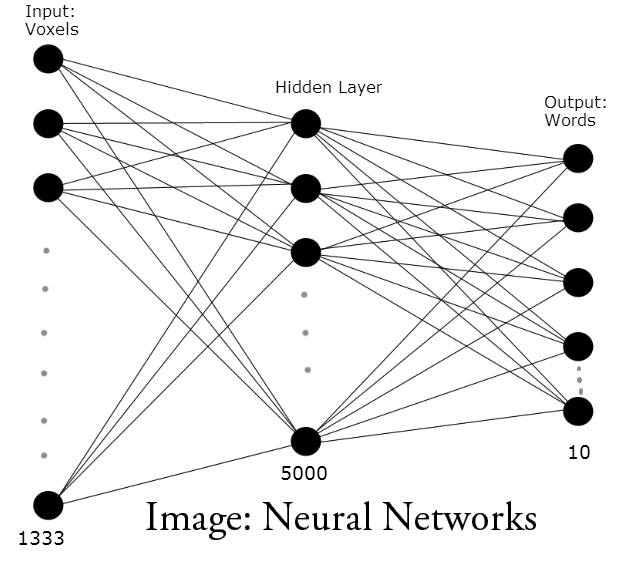
\includegraphics[width=.4\linewidth]{nn.jpg}
  \captionof{figure}{Neural Network Illustration}
  \label{fig:test1}
\end{figure}

\par Our network had an input layer, one 'hidden' intermediate layer, and an output layer. The size of the input layer was equal to the number of feature voxels, the hidden layer size was experimented with for multiple values but set at $n_{hidden} = 5000$, and for the ten words we aimed to predict for, $n_{out} = 10$. These choices were based on optimizations within the restrictions of our computational abilities. A Rectified Linear Unit (ReLU) activation function was used in the hidden layer ($h(z) = \max(0,z)$), and Sigmoid activator from the hidden layer to output layer ($h(z) = \frac{1}{1 + e^{-x}}$). The cost function used was the cost-entropy function, defined as
$$ J = -\sum_{k = 1}^{n_{out}} [y_k\ln h_k(x) + (1-y_k)\ln (1-h_k(x)] $$
We can thus determine the gradient of the cost to travel along as 
\begin{equation} \label{eq1}
\begin{split}
\frac{\partial J}{\partial w} & = \frac{\partial J}{\partial h} \frac{\partial h}{\partial w} \\
 & = -\sum_x \left(\frac{y}{h(x)} - \frac{1-y}{1-h(x)}\right) \frac{\partial h}{\partial w} \\
 & =-\sum_x \left(\frac{y}{h(x)} - \frac{1-y}{1-h(x)}\right) h'(x)
\end{split}
\end{equation}
In the case of ReLU, because it is not a smooth function, we approximate it using the softmax function $h(x) = \ln(1+e^x)$, whose derivative is simply the sigmoid function. For the derivative of the sigmoid function in the output layer, we have $\partial h(x) = h(x)(1-h(x))$. Using the gradient functions, the errors are backpropagated through the network to correct the weights.
\par The TanH function was also tried as an activation function for the input layer, which is a slightly steeper version of sigmoid. The derivative of the tanh function is $\partial h(x) = 1 - h(x)^2$. As the network trains, we also want to slowly decrease the weight of the error modifications, so we define a learning rate $\alpha$
$$ \alpha = \frac{4n}{10ia}$$
where $n$ is the total number of samples, $i$ is the current iteration, and $a$ is the accuracy at the time of learning rate modification (thus favoring lower changes high-accuracy weights). The learning rate was modified every epoch, defined as 100 iterations of stochastic gradient descent.

\begin{figure}
  \centering
  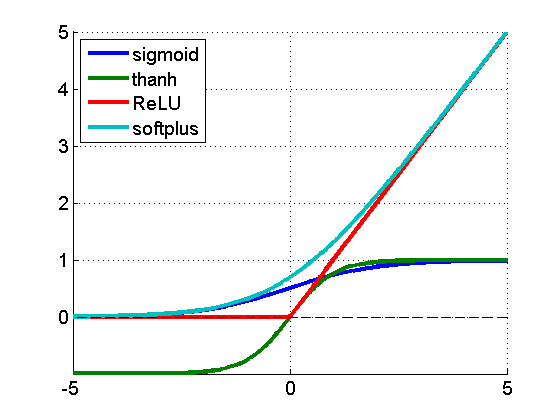
\includegraphics[width=.8\linewidth]{activation_funcs1.png}
  \captionof{figure}{Comparison of Activation Functions}
  \label{fig:test1}
\end{figure}

\par Due to the fully-connected property of layers, that each neuron in each layer inputs/outputs with every neuron in the layers before/after it, large layer sizes increase computational complexity very noticeably. Thus, though we had the 50,000 voxel subset, this was too many neurons for the input layer, and so it was reduced to approximately 5000. Training occurred on approximately 3200 time points, leaving approximately 300 for testing.









